\chapter{Introduction}
\section{Research scope and motivation}


The domain of the proposed thesis is Automated Software Engineering. The thesis will develop methods for the analysis of legacy software systems, focusing on using historical information describing the evolution of the systems extracted from the versioning systems. 
The methods for analysis will integrate techniques based on computational algorithms as well as data-mining. As proof-of-concept, tool prototypes will implement the proposed methods and validate them by extensive experimentation on several cases of real-life systems.\\

\section{Objectives of the thesis}

\hspace{4em}The objective of this doctoral thesis is to investigate and improve methods for filtering logical dependencies extracted from version control systems and to validate the effectiveness of these methods. The filtered logical dependencies are used to enhance key class detection in software systems and to improve software architecture reconstruction, two areas that mostly depend on structural dependencies.

This research proposes techniques for extracting, filtering, and integrating logical dependencies into dependency models. Various metrics will be used to evaluate the impact of incorporating logical dependencies and assess their impact on key class detection and software architecture reconstruction. The goal is to demonstrate that logical dependencies, when appropriately filtered, provide valuable information that can complement or, in some cases, replace structural dependencies.
To achieve this, the following objectives have been established:

\textbf{[O1]}: \textit{Study and analyze the current state of research on logical dependencies to improve their extraction and filtering methods.}

This objective involved the following tasks:
\begin{itemize}
\item \textbf{[T1.1]}: Review existing methods for logical dependency extraction from version control systems.
\item \textbf{[T1.2]}: Identify and evaluate factors that influence the validity of logical dependencies, such as commit size thresholds, minimum co-change occurrences, and comment changes, to develop effective filtering methods.
\item \textbf{[T1.3]}: Based on the observations from T1.2, propose filtering methods for logical dependencies.
\item \textbf{[T1.4]}: Investigate the interplay between logical and structural dependencies to understand their overlap and differences better.
\end{itemize}
The outcomes of this objective [O1] have been published in [A1] and [A2].


\textbf{[O2]}: \textit{Develop a tool for extracting and filtering logical dependencies.}

This objective involved the following tasks:
\begin{itemize}
\item \textbf{[T2.1]}: Designing a tool for extracting logical dependencies based on co-changing entities with different configurable filters.
\item \textbf{[T2.2]}: Implementing and testing the filtering mechanisms by outputting the results in a commonly used format.
\end{itemize}
This objective [O2] has been published and described in more detail in [A1] and [A2], the developed tool being further used in [A3], [A4], and [A5].



\textbf{[O3]}: \textit{Integrate logical dependencies in key class detection.}
This objective involved the following tasks:
\begin{itemize}
\item \textbf{[T3.1]} Extract logical dependencies from version control systems and apply the proposed filter (connection strength).
\item \textbf{[T3.2]} Modify the baseline key class detection tool to incorporate logical dependencies.
\item \textbf{[T3.3]} Evaluate the impact of combining logical and structural dependencies on key class detection performance.
\item \textbf{[T3.4]} Evaluate the impact of using only logical dependencies for key class detection.
\item \textbf{[T3.5]} Investigate the effect of filtering strategies (connection strength with different thresholds) on the key class detection results.
\end{itemize}
The outcomes of this activity [O3] have been published in [A3].

\textbf{[O4]}: \textit{Refine software clustering using logical dependencies.}
This objective involved the following tasks:
\begin{itemize}
\item \textbf{[T4.1]} Review and select suitable clustering algorithms for the experiments.
\item \textbf{[T4.2]} Use only logical dependencies as input for software clustering.
\item \textbf{[T4.3]} Combine logical and structural dependencies as input for clustering algorithms.
\item \textbf{[T4.4]} Investigate the impact of different connection strength filter thresholds on clustering results by using clustering evaluation metrics: MQ and MoJoFM.
\item \textbf{[T4.5]} Analyze the results: logical dependencies alone vs. combined dependencies with varying filter thresholds.
\end{itemize}

The outcomes of this objective [O4] have been published in [A4] and [A5].

\section{Structure of the thesis}

\section{Main Contributions}

\hspace{4em}The principal contributions of this thesis are:  
\begin{itemize}  
    \item proposing methods for filtering logical dependencies extracted from version control systems to improve their reliability and usefulness; this includes introducing a new metric for filtering logical dependencies, called connection strength;  
    \item developing a tool for extracting and filtering logical dependencies;  
    \item integrating logical dependencies into key class detection methodologies and analyzing the impact of different filtering strategies when using logical dependencies both independently and in combination with structural dependencies;  
    \item integrating logical dependencies into software clustering and analyzing the impact of different filtering strategies when using logical dependencies both independently and in combination with structural dependencies; this analysis involves using three distinct clustering algorithms and two evaluation metrics to study the results;  
    \item providing evidence that logical dependencies when appropriately filtered, can improve key class detection and software architecture reconstruction.  
\end{itemize}  

%%%%%%%%%%%%%%%%%%%%%%%%%%%%%%%%%%%%%%%%%%%%%%%%%%%%%

\chapter{Software Dependencies: concepts, applications, and current research}
\label{dep}

\section{Software dependencies overview}

\subsection{Structural dependencies}
\hspace{4em} A dependency is created by two elements that are in a relationship and indicates that an element of the relationship, in some manner, depends on the other element of the relationship \cite{Booch:2004:OAD:975416}, \cite{Cataldo2009SoftwareDW}.

Structural dependencies can be found by analyzing the source code \cite{Sangal:2005:UDM:1094811.1094824}, \cite{CalloArias2011}. 
There are several types of relationships between these source code entities and all those create \textit{structural dependencies}:

\textbf{Data Item Dependencies.}
Data items can be variables, records or structures. A dependency is created between two data items when the value held in the first data item is used or affects the value from the second.


\begin{verbatim}
Example:

int a = 10;
int b = a + 5;  // b depends on a
a = 20;         // changing a doesn't impact b
\end{verbatim}

\textbf{Data Type Dependencies.}
Data items are declared to be of a specific data type. Besides the built-in data types that every programming language has, developers can also create new types that they can use. Each time the data type definition is changed it will affect all the data items that are declared to be of that type. 


\begin{verbatim}
Example:

class Rectangle { int width, height; }
//Change posibility: class Rectangle { int width, height, color; }

Rectangle r = new Rectangle();  
r.width = 5;
r.height = 10;
// Existing code will fail to handle color in case of change
\end{verbatim}

\textbf{Subprogram Dependencies.}
A subprogram is a sequence of instructions that performs a certain task. Depending on the programming language a subprogram may also be called a routine, a method, a function or a procedure. When a subprogram is changed, the developer must check the effects of that change in all the places that are calling that subprogram. Subprograms may also have dependencies with the data items that they receive as input or the data items that they are computing.


\begin{verbatim}
Example:

// First implementation:
class Calculator {
    double calculateArea(double side) {
        return side * side;  
    }
}

// Modified implementation:
class Calculator {
    double calculateArea(double radius) {
        return Math.PI * radius * radius; 
    }
}

Calculator calc = new Calculator();
// Code expecting square area now gets circle area.
double area = calc.calculateArea(5);  

\end{verbatim}





\subsection{Lexical dependencies}

\hspace{4em}Lexical dependencies, similar to structural dependencies, are extracted from the source code. The difference lies in the fact that lexical dependencies focus on finding pairs of entities that are similar (and thus connected) from a linguistic point of view. This means they are based on the textual content and naming conventions used in the code rather than explicit structural relationships. The lexical information about an entity (such as a class or interface) can be extracted from class names, method names, parameter names, code comments, source code statements, and others \cite{lexical-dep}, \cite{lexical-dep-Prajapati}.

For example, a class named \texttt{StructuralDependenciesEvaluator} and a class named \texttt{LexicalDependenciesEvaluation} can be related even if they do not directly share dependencies or their connection is not visible from a structural point of view.

To extract lexical dependencies, the code is tokenized, breaking it down into lexical tokens (e.g., words or symbols). A document containing these tokens is created for each source code file. Each document is then split into different parts, such as a class names part, attribute names part, parameter names part, and others. For instance, the class names part will contain the names of all classes found in the source file.

After the tokenization process and splitting into various parts, the similarity between the two documents is estimated. 

Various methods can be used for similarity calculation, such as:
\begin{itemize}
    \item \textit{Term Frequency-Inverse Document Frequency (TF-IDF):} Weighs the importance of words based on their frequency across documents \cite{lexical-dep}, \cite{corazza2}.
    \item \textit{Cosine Similarity:} Measures the cosine of the angle between two vectors representing the documents \cite{lexical-dep-Prajapati}.
\end{itemize}






\subsection{Semantical dependencies}

\hspace{4em} Podgurski and Clarke define semantic dependencies in source code as follows: if changes in a statement \(s_1\) impact the behavior of another statement \(s_2\), then \(s_1\) and \(s_2\) are \emph{semantically dependent} \cite{Podgurski-semantic}.

Semantic dependencies can be identified from the source code by constructing control flow graphs (CFGs). A control flow graph is a directed graph \(G = (V, E)\), where:
\begin{itemize}
    \item \(V\) is the set of vertices representing program statements (e.g., assignments, method calls, conditions),
    \item \(E\) is the set of edges representing possible transfers of control between statements.
\end{itemize}

A vertex \(u \in V\) is semantically dependent on a vertex \(v \in V\) if changes in \(v\) determine changes in \(u\).

In object-oriented (OO) systems, semantic dependencies are dependencies that are not visible in the static structure of the code. There is no direct reference between two entities (e.g., classes or interfaces), but changes in one entity impact the behavior of the other \cite{Neto-semantic-dep, Capiluppi-semantic-dep, Poshyvanyk2009}. 


\textit{Example:}

Let \(A\) a class that uses an object of type \(I\), and let \(B\) a class that implements \(I\). For example, class \(A\) calls a method \texttt{performAction()} via an interface \(I\), while class \(B\) implements the \texttt{performAction()} method.

If \(B\) changes its implementation of \texttt{performAction()}, the behavior of \(A\) might also change when it uses \(B\). This means that \(A\) and \(B\) are semantically dependent.



\subsection{Logical dedependencies}
\hspace{4em} \textit{Logical dependencies} (also known as logical coupling) can be discovered through software history analysis. They reveal relationships between entities that are not always present in the source code's static structure (i.e., structural dependencies).

Software engineering practice has shown that sometimes modules without explicit structural dependencies still appear to be related. \textit{Co-evolution} represents the phenomenon where one component changes in response to changes in another component \cite{Yu:2007:UCC:1231330.1231370, Cataldo2009SoftwareDW}. Such changes can be found in the software history maintained by version control systems. Gall et al. defined \textit{logical coupling} as the occurrence of modules that \emph{repeatedly} update together during the evolution of the software system \cite{Gall:1998:DLC:850947.853338, Gall:2003:CRH:942803.943741, 6606615}.

The concepts of logical coupling and logical dependencies have been applied in different analysis tasks related to software changes: for software change impact analysis \cite{1553643}; for identifying potential ripple effects caused by software changes during maintenance and evolution \cite{DBLP:conf/issre/OlivaG15, Oliva:2011:ISL:2067853.2068086, Poshyvanyk2009, posh2010}; and for exploring their link to defects \cite{wiese, Zimmermann:2004:MVH:998675.999460}.

An in-depth analysis of how logical dependencies are identified within the versioning system and their applications is provided in Section \ref{ld-intro}.



\subsection{Additional dependencies}

\hspace{4em} Besides the dependencies mentioned above, there are many other types of dependencies, such as temporal, package, external, and several others.

\textit{Temporal dependencies} represent a type of dependency where certain operations in the code must occur in a specific order. These operations may belong to the same software component or span across different parts of the system \cite{Cataldo2009SoftwareDW}.

\begin{verbatim}
Example:

var file = new File();
file.open("example.txt");
file.readContents();
file.close();
\end{verbatim}

In this example, there is a temporal dependency between the \texttt{open}, \texttt{readContents}, and \texttt{close} methods. The \texttt{readContents} method cannot function correctly unless the \texttt{open} method is called first to open the file. Similarly, the \texttt{close} method should be called after \texttt{readContents} to release the file resources.


\textit{Package dependencies} refer to the relationships between different software packages, usually managed using package managers \cite{dep-package}.

\textit{External dependencies} are the relationships between a software system's code and components outside the system, such as third-party services, libraries, APIs, or the programming language itself \cite{dep-external}.






\section{Software change and version control systems}

\subsection{Software change}
\label{change}

\hspace{4em}Software systems have distinctive stages during their life: initial development, evolution, servicing, phase out, and close down \cite{Software-life-cycle}, \cite{model-bennett}.

In the \textit{evolution stage}, iterative changes are made. By changes, we mean additions (new software features), modifications (changes of requirements or misunderstood requirements), or deletions. There are two main reasons for the change: the software team's learning process and new requests from the client.

Suppose new changes are no longer easy to be made or are very difficult and time-consuming. In that case, the software enters the \textit{servicing stage}, also called aging software, decayed software, and legacy \cite{Software-life-cycle}, \cite{363157}.

The main difference between changes made in the evolution and servicing stages is the effort to make changes. In the evolution stage, software changes are made easily and do not require much effort, while in the servicing stage, only a limited number of changes are made and require a lot of effort, so they are time-consuming \cite{Bennett, Rajlich, FoSEReverseEngineering}.

The change mini-cycle consists of the following phases \cite{810308}:
\begin{itemize}
\item Phase 1: The change request. This usually comes from the software users, and it can also be a bug report or a request for additional functionality.
\item Phase 2: The planning phase includes program comprehension and change impact analysis. Program comprehension is a mandatory prerequisite of the change, while change
impact analysis indicates how costly the change will be. \cite{Bohner}
\item Phase 3: The change implementation, restructuring for change, and change propagation.
\item Phase 4: Verification and validation.
\item Phase 5: Re-documentation.
\end{itemize}

Understanding these phases is important for ensuring the software system remains maintainable and reliable throughout its lifecycle.


\subsection{Version control systems}

\hspace{4em}Software evolution implies change which can be triggered either by new feature requests or bug reports \cite{articleEvolution}. As presented also in section \ref{change}, one phase of the change mini-cycle consists of change implementation and propagation (changing source code files). 
Usually, developers use version control when it comes to software development. Version control is a system that records changes to a file or set of files over time so that developers can recall specific versions of those files later \cite{svn}.
Distributed version control systems (such as Git, Mercurial, Bazaar or Darcs) allows many developers to collaboratively develop their projects \cite{7471284}.

Below, we will review some of the operations supported by versioning systems. The operation names in the following text are specific to Git, as Git is the version control system used for data collection in the current work. However, similar operations exist in other versioning systems; for example, Subversion (SVN) and Mercurial also provide operations such as branching, merging, and committing changes.

\textbf{Repository}

A repository serves as a centralized storage location for project files. The entire codebase of a project can be stored within a single repository or be split into a main repository and various modules stored in multiple repositories. Git repositories can be hosted on numerous platforms, such as GitHub, GitLab, Bitbucket, and others.

It is important to differentiate between Git and Git hosting services. Git is a version control system that allows developers to download and modify code on their local devices while hosting services like GitHub provide platforms for teams to host projects that utilize Git \cite{git}, \cite{github}.

\textbf{Commits}

Committing is an operation that allows developers to record the latest changes to the codebase in the repository. A commit saves the current state of the code, including changes made since the last commit.

The changes tracked include:

\begin{itemize}
\item \textit{Additions:} New files or lines of code created.
\item \textit{Modifications:} Updates to existing lines of code or files.
\item \textit{Deletions:} Removal of files or lines of code that are no longer needed.
\end{itemize}

The \textit{push} operation uploads these changes to the remote repository on the hosting service.

A unique identifier, also known as a commit hash, is assigned to each commit. This hash allows developers to track specific changes or revert to earlier code versions. When a developer commits the changes, a commit message is required. This message serves as documentation for the changes, enhancing code traceability and maintainability \cite{git}.

Figure~\ref{fig:gitflow} illustrates how changes are made to the code over time through commits, starting from the initial commit to the latest version.

\begin{figure}[h!]
\centering
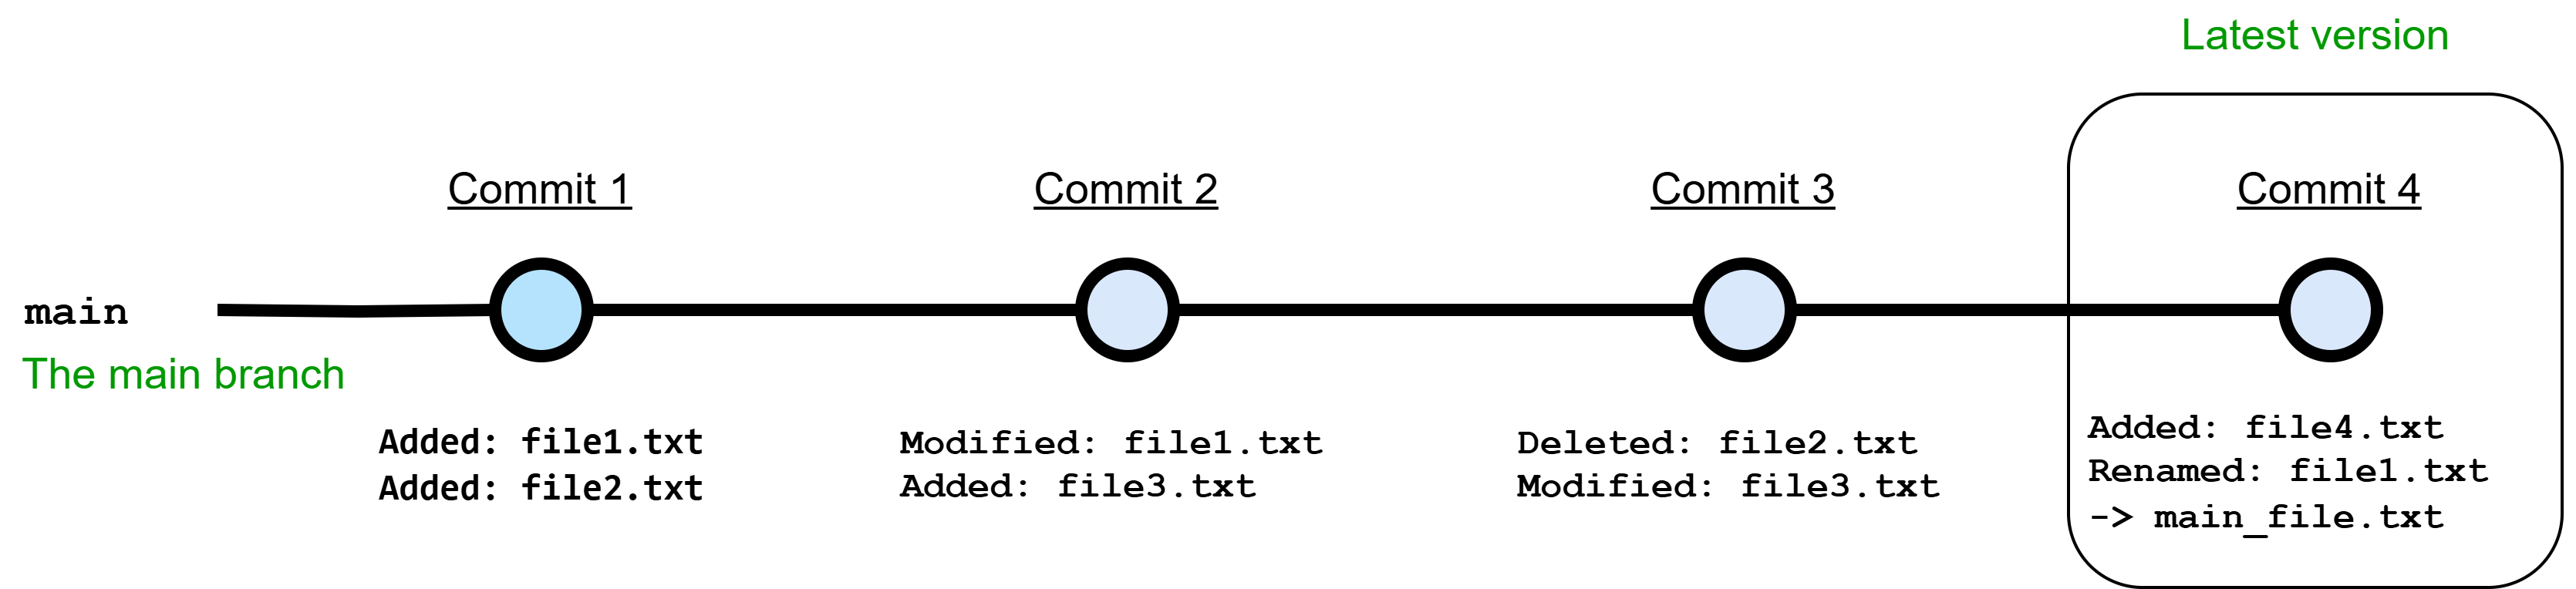
\includegraphics[width=\textwidth]{gitflow.png}
\caption{Tracking changes through commits.}
\label{fig:gitflow}
\end{figure}

\textbf{Branches and Merging}

By default, every repository comes with a main (or master) branch. This branch represents the central timeline for code changes and serves as the main integration point for stable code. Other branches can be created for parallel development from this branch.

Branches allow developers to encapsulate changes without affecting the main branch. In most software projects, it is standard practice for developers to use branches for development, with the main branch being locked for direct commits. Changes to the main branch can be integrated through merges from other branches.

Software projects often have multiple branches running in parallel, including branches from other branches. The main branch is not the only branch that supports branching; any branch can be a base for creating other branches.

The operation of integrating changes from one branch into another (usually into the main branch) is called \textit{merging}.

There are three main types of merges in Git \cite{git}:

\begin{itemize}
    \item \textit{Git Merge:} This is the most commonly used type of merging. It creates a new merge commit that combines all the changes from the branch being merged. Additionally, it retains the history of all the individual commits in the branch.
    \begin{verbatim}
    git checkout main
    git merge feature-branch
    \end{verbatim}

    \item \textit{Git Rebase and Merge:} This operation is typically used when the branch contains a single commit or a small number of commits. It moves all the commits from the source branch to the top of the target branch. The main disadvantage of this operation is that it rewrites the commit history.
    \begin{verbatim}
    git checkout feature-branch
    git rebase main
    git checkout main
    git merge feature-branch
    \end{verbatim}

    \item \textit{Git Squash and Merge:} This operation compresses all commits from the source branch into a single commit before merging it into the target branch. It results in a cleaner commit history but has the disadvantage of losing individual commits from the source branch.
    \begin{verbatim}
    git checkout main
    git merge --squash feature-branch
    git commit
    \end{verbatim}
\end{itemize}


Figure~\ref{fig:merging} illustrates the differences between these three types of merging. 

\begin{figure}[h!]
    \centering
    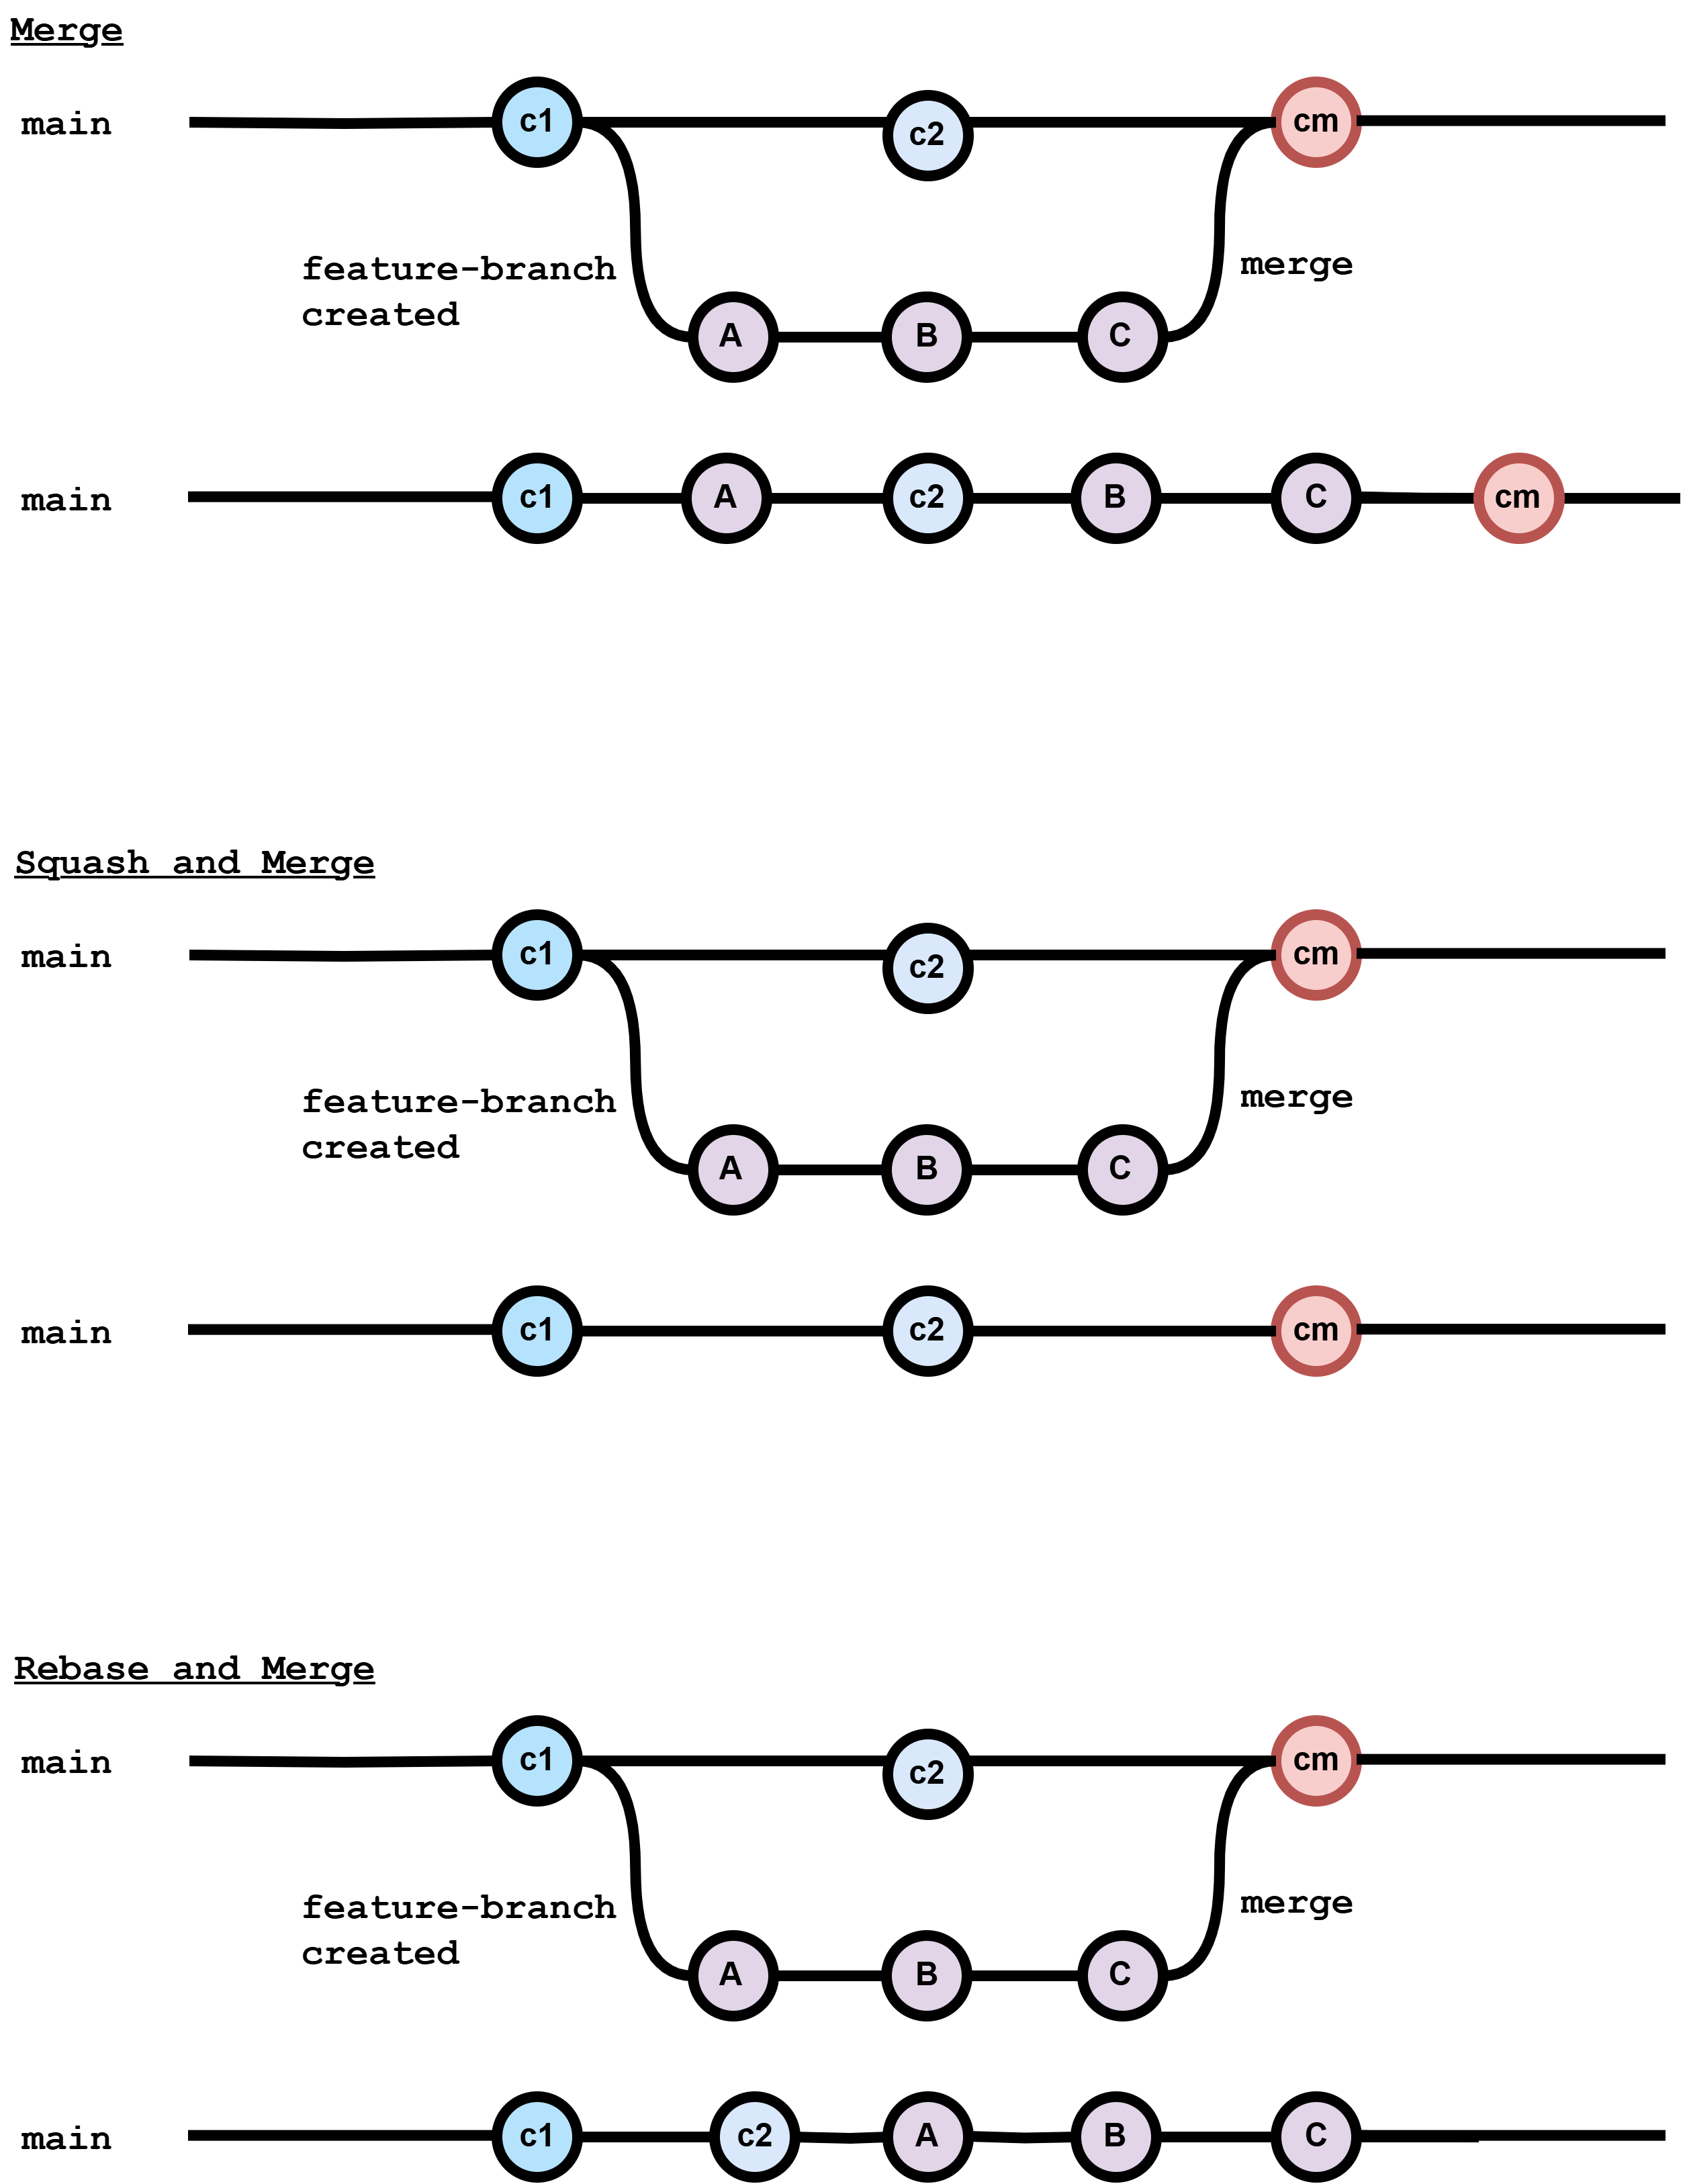
\includegraphics[width=\textwidth]{merging.png}
    \caption{Comparison of Git merge types.}
    \label{fig:merging}
\end{figure}

\textbf{Tagging}

Another helpful operation in Git is tagging. Developers use the tagging operation to mark a specific code version at a particular commit. This is usually done for important milestones, such as a new release version or a stable build \cite{git}.

Tags provide a way to create a human-readable reference to a specific commit (e.g., \texttt{v1.0.0}), as the commit hash can be hard to remember (e.g., \texttt{a1b2c3d4e5f6g7h8i9})

Git supports two types of tags:
\begin{itemize}
    \item \textit{Lightweight Tags:} Simple references to a commit that do not contain any additional metadata.
    \item \textit{Annotated Tags:} These include additional metadata such as the author's name, date, and message, making them more suited for marking releases.
\end{itemize}



\section{Current status of research on logical dependencies}
\label{ld-intro}

\subsection{Logical dependencies in software systems}

\hspace{4em}The versioning system stores the long-term change history of every file in a project. Each change made by an individual at a specific point in time is recorded as a commit \cite{7471284}. This historical data provides insights into how software components evolve over time. Logical dependencies, also known as evolutionary coupling or co-changes, are derived from patterns of co-evolution, where one component changes in response to changes in another \cite{Yu:2007:UCC:1231330.1231370, 5166450, Beck:2011:CMC:2025113.2025162}.

Gall \cite{Gall:1998:DLC:850947.853338, Gall:2003:CRH:942803.943741, 6606615} identified \textit{logical coupling} as the relationship between two modules that repeatedly change together during the historical evolution of a software system. Logical dependencies can be expressed at two levels of abstraction: module-level \cite{LD-module-new} and file/class-level \cite{Gall:2003:CRH:942803.943741, inproceedings-gall}.

Several tools have been developed to detect and use logical dependencies. For instance, the \textbf{ROSE} tool, developed by Zimmermann et al. \cite{Zimmermann:2004:MVH:998675.999460}, mines version histories to suggest related code changes based on historical coupling between software entities. ROSE can predict 26\% of further files to be changed and 15\% of the functions or variables involved in future modifications.

Kagdi et al. \cite{article-Kagdi-commit, msr-kagdi} developed \textbf{sqminer}, a tool based on the SPADE (Sequential Pattern Discovery Algorithm) to mine sequences of file changes for software change prediction. They also proposed an approach that combines conceptual couplings (derived from textual analysis of source code comments and identifiers) with logical dependencies (mined using the sqminer tool) to enhance software change impact analysis \cite{article-Kagdi-commit}.

Moonen et al. \cite{Moonen-commit, article-Moonen, 7476643} proposed an algorithm called \textbf{Tarmaq} that analyzes evolutionary coupling for predicting co-changes. Their results demonstrated that Tarmaq achieves better performance than the ROSE tool. Similarly, Mondal et al. \cite{HistoRank} developed \textbf{HistoRank}, an algorithm that uses five different ranking strategies for prioritizing and filtering co-changes.

As shown above, logical dependencies have been widely used in co-change prediction. Additionally, they have been used for various other purposes, such as detecting code clones \cite{Mandal-clones}, identifying buggy code \cite{buggy-code}, evaluating the impact of software changes \cite{1553643}, and identifying potential ripple effects caused by software changes during maintenance and evolution \cite{DBLP:conf/issre/OlivaG15, Oliva:2011:ISL:2067853.2068086}.

Despite their utility, logical dependency usage presents several challenges. One significant issue is the large volume of information generated during extraction, which must be processed and filtered to remove noise \cite{Coupling-Lanza, articleEvolution, Shtern:2012:CMS:2332427.2332428}. For instance, \textit{Oliva and Gerosa} \cite{Oliva:2011:ISL:2067853.2068086} found that the set of co-changed classes was much larger than the set of structurally coupled classes. At least 91\% of logical dependencies involve files that are not structurally related. This implies that not all change dependencies are linked to structural dependencies and that other factors may cause software artifacts to be change-dependent.

Ajienka and Capiluppi also explored the interplay between the logical and structural coupling of software classes. In \cite{DBLP:journals/jss/AjienkaC17, DBLP:journals/ese/AjienkaCC18}, they conducted experiments on 79 open-source systems. For each system, they identified the sets of structural dependencies, logical dependencies, and the intersections of these sets. They studied the overlap between these dependencies, concluding that not all co-changed class pairs (logical dependencies) are also linked by structural dependencies. Another observation, which was not deeply investigated by the authors in \cite{DBLP:journals/jss/AjienkaC17, DBLP:journals/ese/AjienkaCC18}, is the ratio between the total number of logical dependencies and structural dependencies in software systems. Based on their raw data, the average ratio across all analyzed projects is approximately 12.

Applications based on dependency analysis could benefit from incorporating non-structural dependencies alongside structural ones. For example, works that investigate various methods for architectural reconstruction \cite{SoraConti, SoraSem13, PagerankENASE}, which rely mostly on structural dependency data, could enhance their dependency models by including logical dependencies.

Logical dependencies should integrate harmoniously with structural dependencies. Valid logical dependencies should not be excluded from the model, but structural dependencies should also not be overwhelmed by questionable logical dependencies. Therefore, to effectively incorporate logical dependencies into dependency models, co-changes must be filtered to remain only with a reduced and relevant set of valid logical dependencies.




\subsection{Existing filtering techniques}

\hspace{4em}Currently, there are no fixed rules for filtering extracted class co-changes to ensure they form a set of valid logical dependencies. Most studies using or investigating logical dependencies have applied various filtering techniques to the extracted co-changes. Below are some of the most commonly used filtering methods cited in the literature.


\textbf{Commit Size}  

One of the most frequently used filters for co-change extraction is the commit size filter. Commit size refers to the number of code files modified in a specific commit. Large commits, which involve a significant number of files, are often the result of non-code-related tasks, such as branch merges or folder renaming. These operations can introduce irrelevant co-changing pairs of entities, adding noise. To solve this issue, commit size filtering is applied to the information extracted from version control systems.

\textit{Ajienka and Capiluppi} \cite{DBLP:journals/jss/AjienkaC17} established a threshold of 10 files, discarding all commits with more than 10 modified files from their research.

\textit{Kagdi et al.} also applied the same threshold, excluding commits with more than 10 source files from their analysis.

\textit{Ying et al.} \cite{Ying-co-change} set a higher threshold, excluding transactions involving more than 100 files.

\textit{Zimmermann et al.} \cite{Zimmermann:2004:MVH:998675.999460} configured the ROSE tool to exclude changes involving more than 30 files.

\textit{Moonen et al.} \cite{Moonen-commit} considered seven different transaction filtering sizes: 2, 4, 6, 8, 10, 20, and 30 (with 30 being the upper bound suggested by Zimmermann) and recommended excluding transactions larger than 8 files.

However, most of the works presented above do not discuss how the thresholds were chosen, nor do they analyze the impact of different threshold values on the quantity and quality of the data extracted.


\textbf{Support and confidence}

Filtering based only on commit size is not enough. While this type of filtering can reduce the total number of extracted co-changes, it does so without guaranteeing that the remaining co-changes are more relevant.

Unrelated files can sometimes be updated in small commits due to human error. For instance, a file that was omitted from the current commit may be committed in the next commit together with some unrelated files. Such scenarios can introduce co-changing pairs that are not genuinely linked. To address this problem, a filter based on the occurrence rate of co-changing pairs should be applied. Co-changing pairs that occur multiple times are more likely to be dependent than those that appear only once \cite{b4}.

Zimmermann et al. \cite{Zimmermann:2004:MVH:998675.999460} introduced the support and confidence metrics to measure the significance of co-changes based on the occurrence rate of co-changing pairs.

The \textit{support metric} of a rule $(A \rightarrow B)$, where A is the antecedent and B is the consequent of the rule, is defined as the number of commits (transactions) in which both entities are changed together.

The \textit{confidence metric} of $(A \rightarrow B)$, as defined in Equation \eqref{eq:confidence}, focuses on the antecedent of the rule and is the number of commits together of both entities divided by the total number of commits of (A).

\begin{equation}
\text{Confidence}(A \rightarrow B) = \frac{\text{Nr. of commits containing } A \text{ and } B}{\text{Nr. of commits containing } A}
\label{eq:confidence}
\end{equation}


The support metric represents the frequency of changes for an association rule and can take values from 0 to infinity. On the other hand, the confidence metric is defined within the interval [0, 1]. As in Equation \eqref{eq:confidence}, the confidence metric measures the likelihood of a co-change. It can never exceed 1 because $\text{Commits}(A \cap B)$ is always a subset of $\text{Commits}(A)$.


 For example, consider the case where entity $A$ is modified in 10 commits and entity $B$ is modified together with $A$ in 7 of those commits. The confidence is then:

\[
\text{Confidence}(A \rightarrow B) = \frac{7}{10} = 0.7.
\]

If $A$ and $B$ are always modified together in all 10 commits involving $A$, the confidence would be:

\[
\text{Confidence}(A \rightarrow B) = \frac{10}{10} = 1.
\]



Many studies have used the support and confidence metrics. Zimmermann et al. \cite{Zimmermann:2004:MVH:998675.999460}, in their ROSE tool, used different combinations of minimum support and confidence thresholds. They applied three minimum support thresholds, 1, 3, and 5, together with confidence thresholds ranging from 0.1 to 0.9, to predict future changes in software systems.

Ying et al. \cite{Ying-co-change} recommend potentially relevant source code to developers during modification tasks. The support thresholds in their study vary based on the analysis, ranging from 5 to 30 (5, 10, 15, 20, 25, 30). For confidence, Ying et al. chose not to use this metric, as they consider it misleading when some files are changed much more frequently than others.

Kagdi et al. \cite{article-Kagdi-commit}, in their studies on software change prediction, used minimum support thresholds of 1, 2, 4, and 8. For confidence, they considered all possible values greater than zero.

Mandal et al. \cite{Mandal-clones}, in their study on detecting clones and analyzing their evolution, developed a tool called MARC (Mining Association Rules among Clones). The tool detects code clones and ranks their change-proneness based on support and confidence values. In their experiments, they applied a minimum support threshold of 1.

Ajienka and Capiluppi \cite{DBLP:journals/ese/AjienkaCC18}, in their study on the interplay between logical and structural dependencies, used a support threshold of 0.01 and a confidence threshold of 0.1.



\textbf{History length and age}

Moonen et al. investigated the influence of history length (the number of analyzed transactions) and history age (the number of transactions that have occurred since the last co-change) when mining evolutionary coupling. Their study, which analyzed over 540,000 commits, found no evidence to support the idea that there is an upper limit to the amount of history that can be used for mining evolutionary coupling before outdated knowledge starts to negatively affect the quality of the extracted information \cite{article-Moonen}.


\section{Applications of software dependencies}
\label{app}

\hspace{4em}This section reviews several applications of software dependencies (e.g., structural, lexical, semantical, logical dependencies). These dependencies play an important role in various software engineering tasks, architecture reconstruction, clone identification, and more. 


\textbf{Architecture reconstruction.}
Currently, software systems contain tens of thousands of lines of code and are updated daily by multiple developers. The software architecture is important for understanding and maintaining a system. Often, code updates are made without checking or updating the architecture.

These kinds of updates cause the architecture to drift from the reality of the code over time. Therefore, reconstructing the architecture and verifying if it still matches the actual implementation is important \cite{RecoverySartipi, model-bennett, Kalliamvakou2016}. Architecture reconstruction has mainly been done using structural dependencies \cite{sar}, \cite{PagerankENASE}, \cite{Bass-archreconstruction}, but recent works also include semantical and logical dependencies \cite{lexical-dep}, \cite{corazza2}, \cite{maletic}.

\textbf{Identifying Clones.} 
Research suggests that a considerable portion (around 5-10\%) of the source code in large-scale software is duplicate code (“clones”). Source code is often duplicated for a variety of reasons: programmers may simply reuse a piece of code by copying and pasting, or they may “reinvent the wheel” \cite{ClonesMayrand}, \cite{clones}. Detection and removal of clones can significantly decrease software maintenance costs \cite{CloneDetection}, \cite{cloneKamiya}.

Structural dependencies can be used to detect code clones. For example, Cordy and Roy created the NiCad tool, which receives the entire code base of a project as input to detect project clones \cite{clones-nicad}. The same authors also used versioning system information to link clones to bug-fix commits from the versioning system \cite{clones-nicad-git}. Other researchers have used semantic dependencies and machine learning techniques to identify clones \cite{clones-ml}, while others have used lexical dependencies extracted from code comments \cite{clones-comments}.

\textbf{Code Smells.}  
Fowler \ defined code smells cite{bookFowler} as patterns generally associated with bad design and poor programming practices. Originally, code smells were used to identify areas in software that may require refactoring \cite{articlesmells}. Studies have found that code smells can impact software comprehension and increase changes and faults in the system \cite{5741260}, \cite{5328703}, \cite{articlefault-proneness}.

Examples of code smells include:

\begin{itemize}
    \item \textbf{Large Class:} A class with many fields and methods, making it difficult to maintain or understand.
    \item \textbf{Feature Envy:} Methods that access more methods and fields of another class than of their class.
    \item \textbf{Data Class:} Classes that contain only fields and no meaningful functionality.
    \item \textbf{God Class:} A class that centralizes too much responsibility, often not respecting the Single Responsibility Principle.
    \item \textbf{Refused Bequest:} A subclass that inherits many fields or methods from its parent but leaves them unused.
    \item \textbf{Parallel Inheritance:} Every time a subclass is added to one class, a subclass must also be added to another class.
    \item \textbf{Shotgun Surgery:} A single change requires modifications in multiple classes.
\end{itemize}

Code smell detection approaches often use structural information extracted from static code analysis. For example, Marinescu \cite{Marinescu} proposed a method to identify smells like God Class and Data Class based on structural metrics. Recent works have used machine learning algorithms in combination with structural metrics to improve the detection of code smells \cite{code-smell-ml, PALOMBA20181}.

Certain smells, however, are more effectively detected using information from versioning systems, which capture logical dependencies. For instance, smells like \textit{Parallel Inheritance} and \textit{Shotgun Surgery} have been successfully identified by analyzing co-change patterns in version control systems \cite{6963448}.


\textbf{Key Classes.} The concept of key classes was first introduced by Zaidman et al.\ \cite{ZaidmanJurnal}, referring to classes found in documents that provide an architectural overview of the system or an introduction to its structure. Tahvildari and Kontogiannis provided a more detailed definition of the key classes concept: \textit{“Usually, the most important concepts of a system are implemented by very few key classes which can be characterized by specific properties. These classes, which we refer to as key classes, manage many other classes or use them in order to implement their functionality. The key classes are tightly coupled with other parts of the system.”}~\cite{Tahvildari2004ImprovingDQ}.

Key class identification can be performed using different algorithms with various inputs. Most of the research is based on using structural dependencies~\cite{PagerankENASE}, \cite{enase15}, \cite{PagerankSACI}, \cite{Finding-key-classes}, \cite{ZaidmanJurnal}, \cite{rocclasification}, class diagrams~\cite{6676885}, or \textit{dynamic dependencies} obtained through runtime analysis \cite{ZaidmanJurnal}. 

\textbf{Comprehension.}  
Software comprehension is the process of gaining knowledge about a software system. An increased understanding of the software system helps activities such as bug correction, enhancement, reuse, and documentation \cite{Comprehension}, \cite{1199197}. 

Previous studies show that the proportion of resources and time allocated to maintenance activities can vary from 50\% to 75\% \cite{articleLientz}. Within the maintenance process, the biggest effort is dedicated to understanding the system.

To support software comprehension, various tools have been developed to help this process. For example, the COSPEX tool developed by Gupta et al. uses source code analysis to help novice developers better comprehend their tasks \cite{Comprehension-Gupta}. Şora proposes a tool that uses structural dependencies and graph-based ranking to generate an executive summary highlighting the most important classes in the software system \cite{enase15}.


\textbf{Fault Localization.}

Debugging software is an expensive and mostly a manual process. Among all debugging activities, fault localization is the most time-consuming task \cite{articleDebugging}. 

Software developers typically locate faults in their programs through a manual process. This process begins when developers observe failures in the program. They select a dataset to inject into the system, which is a set of data likely to replicate previous failures or trigger new ones, and set breakpoints using a debugger. They then monitor the system's state until a failure occurs and backtrack from the failure state to identify the root cause of the fault \cite{fault-localization, program-failures}. 

Several tools and methods have been developed to support in the fault localization process. A commonly used technique is running coverage tests to evaluate the likelihood of faults in different parts of the source code. Code statements or methods having more failing tests than passing tests are labeled more likely to contain faults. An example of such a tool is GZoltar, developed by Campos et al. \cite{fault-gz}. 

More recent studies have suggested enhancing fault localization techniques by incorporating information from versioning systems in addition to source code analysis. Wen et al. empirically demonstrated that versioning system data could improve fault localization. Their approach identifies code entities modified by more "bug-inducing commits" than regular commits, labeling them as potential fault sources \cite{fault-versioning}.


\textbf{Defect Prediction.}

Fault localization is the process of identifying elements responsible for software failures reported by users or discovered by developers. Defect prediction, on the other hand, predicts elements that are likely to be fault-prone before faults occur. Due to this difference, fault localization and defect prediction are studied as two separate research areas \cite{error-prone, fault-survey}.  

Research has shown that modules or entities most likely to contain defects can be identified based on structural metrics (e.g., lines of code, cyclomatic complexity) and versioning system data (e.g., frequency of changes, modified code in a source file) \cite{67595}, \cite{1702015}.
